\documentclass[12pt,a4paper]{scrartcl}

\usepackage[sort&compress]{natbib}
\usepackage[english]{babel}
\usepackage{booktabs, times, rotating, tabularx, tabulary, multirow, authblk, microtype, amsmath, setspace, marvosym, graphicx, fullpage}
\doublespacing


%opening
\title{The Value of Highway Noise Abatement Measures}
\author{Duco de Vos\thanks{d.w.de.vos@student.vu.nl}}
\affil{Vrije Universiteit Amsterdam}

\begin{document}
	
	\maketitle
	
	\begin{abstract}
	
	In this thesis I estimate the causal effect of noise barrier construction, speed limits, and implementation of silent tarmac on transaction prices of residential properties that suffer noise exposure. I employ the hedonic approach, using data provided by the ``Dutch Association of Real Estate Agents" (NVM), and the Dutch Highway authority (Rijkswaterstaat). With the use of Geographic Information Systems the housing and infrastructure data were linked. The results indicate that different types of noise abatement measures have different effects on housing prices. The most effective noise abatement measures, as measured by the hedonic approach, are the construction of ``berm barriers'' and setting a stricter speed limit. 
		
	\end{abstract}
	
	\section{Introduction}
	\label{sec:intro}
	
	Transport noise is a costly affair. Substantial noise levels can cause annoyance, stress and illness. According to a European report \citep{CEDelft2011}, the external cost of noise induced by road transport in Europe\footnote{EU27 excluding Malta and Cyprus, including Norway and Switzerland.} amounts to \EUR17 Billion annually. In Europe the Environmental Noise Directive\footnote{European Commission, 2002. Environmental noise directive 2002/49/EG.} aims to reduce harmful noise exposure of citizens. Without specifying limit noise values, this directive still gives governments the incentive to devise policy measures against noise. In the Netherlands local noise limit values are specified for highways\footnote{Chapter 11.3, Wet Milieubeheer, 2012}. Using a combination of acoustical models and measurements, the Dutch highway authority (Rijkswaterstaat) determines if these limit values are reached and, if so, which measures should be taken to reduce noise-nuisance \citep{DeVos2015}. The main goal of noise abatement measures is to minimize the external costs of noise, in the absence of a market for tranquillity. In the Netherlands the negative external effects of road noise may, partly, be mitigated by road and fuel taxes, in combination with policy measures such as vehicle regulation, silent tarmac, traffic-management systems, noise barrier walls, and ultimately housing insulation\citep{RIVM2001}. 
	
	The existence of demand for road noise mitigating measures and the costly supply of these policy instruments implies a trade-off between accepting noise levels and employing resources to hamper noise generation and/or propagation. Cost-benefit Analysis, which results in the net present value of all (social) costs and benefits involved in a project, is often employed in the decision-making process on whether or not to use a certain policy instrument. The absence of a market for tranquillity implies a need for "Willingness to pay" estimations for noise reduction measures, as the CBA technique requires all costs and benefits of a project to be measured in the same metric, usually money.
	
	Although there is a strand of economic literature that deals with the negative effects of highway noise (see \cite{Nelson1982,Nelson2008,Bateman2001}), generally these studies estimate WTP values for noise reduction in dB(a), and little emphasis is put on the effectiveness of employed abatement measures. In this Master Thesis I investigate the causal effect of highway noise abatement measures with a clear local extent (noise barriers, silent tarmac and, to some extent, speed limits), on transaction prices of residential properties in the immediate vicinity of the affected roads. I employ a panel data approach, with fixed effects for relatively small areas, using data for the years 2005-2013. This work is structured as follows: section \ref{sec:litrev} gives a dense literature overview, section \ref{sec:method} describes the empirical modeling framework, in section \ref{sec:data} I discuss the different data and their sources, section \ref{sec:results} presents the estimation results and section \ref{sec:conclusion} concludes.
	
	\section{Literature review}
	\label{sec:litrev}
		
		\subsection{Noise abatement policy}	
	
		Road noise is regarded as an external cost, because motorists do not (fully) take into account the noise nuisance they impose on others by driving on a road, mainly because of the absence of a market for tranquillity \citep{Nelson2008}. This market failure is a ground to devise policy measures to minimize the social costs of noise, up to the point where the marginal costs of abatement (e.g. construction costs of noise barriers, induced effects of lower speed limits) equal the marginal benefit of abatement (i.e. the marginal aggregate willingness to pay for noise reduction). In simple cases the problem might be solved by assigning property rights, although this measure seems more plausible in an aviation context than in a road traffic context \citep{Gillen2003}, because of the more local extent. Another "first-best" solution would be to charge motorists the marginal external costs they impose on others, by instituting a road pricing scheme. Nowadays electronic road pricing (ERP) schemes can be used to charge motorists a tax that can be differentiated along several dimension (trip duration, vehicle type, etc.) that reflect the external costs they impose\citep{Verhoef1995}. Social and political issues, however, prevent such systems from being introduced widely. 
	
		\begin{figure}[h]
			\caption{Factors causing adverse noise effects, based on \cite{Nijland2003}}
			\label{fig:NoiseEffects}
			\centering
			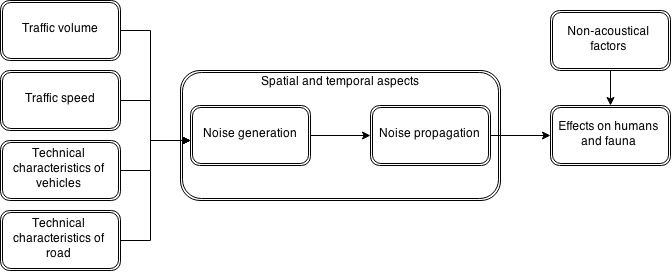
\includegraphics[width=\textwidth]{Graph0}
		\end{figure}
	
		The Dutch government uses an array of policy tools to tackle the problem of road noise, next to general road- and fuel taxes. The amount of noise a vehicle produces depends on the vehicles' technical characteristics (motor, tyres, etc.), driver characteristics (speed and driving style), and on the type of road surface \citep{Nijland2003} (see Figure \ref{fig:NoiseEffects}). Source based policy measures affect noise generation: restrictions on vehicle characteristics are made at the EU level\footnote{European Commission, 2007.  Vehicle type approval framework directive 2007/46/EC.}, decisions on implementation of silent tarmac, speed limits and traffic management systems are made at a more local level. Next to source based measures, the Dutch government also tries to hamper noise propagation in various instances, mainly through the construction of noise barriers. Measures directed at noise generation are generally more cost-effective than noise propagation measures \citep{DenBoer2007}. The efficiency of noise abatement measures is hardly studied in an economic context, \cite{Nijland2003} evaluate the implementation of silent tires and silent tarmac in the Netherlands in a CBA setting, using information based on several meta-analyses and expert reports.
	
		\subsection{Willingness-to-pay estimation}

		Economic valuation of (infrastructure-) externalities is done in two distinct ways: revealed preference and stated preference (SP) methods. Both these methods result in willingness-to-pay values for the public good, or public bad, in question. Revealed preference methods, such as the hedonic pricing (HP) method, use real life data on choices made in markets that are complementary to externality avoidance (often the market for housing); stated preference methods, such as the contingent valuation method, construct a market by means of survey techniques \citep{Nelson2008}. I will discuss the details of the HP method (see \cite{Bristow2014} for a recent meta-analysis on transport noise valuation using stated preference methods). 
		
		The hedonic pricing method was introduced by \cite{Rosen1974}, defining hedonic prices as
		\begin{quote}``\dots implicit prices of attributes (\dots) revealed (\dots) from observed prices of differentiated products and the specific amounts of characteristics associated with them."\end{quote} 
		This means that, in hedonic pricing models, the willingness-to-pay for a product is subdivided in terms of product characteristics and attributes. Theoretically, a premium for a certain noise abatement measure can be obtained by analysing the market values of identical houses in a location with, and a location without a certain applied measure, for instance a noise barrier. In literature concerning road noise, a discount for a noisy environment is often calculated, following the same principle.
		
		The 4 main assumptions for the operation of hedonic pricing analysis are defined by \cite{Bateman1993}:
		\begin{enumerate}
			\item Aggregate willingness-to-pay reflects the social benefit.
			\item Environmental quality changes are perceivable, and they affect the future benefits from owning a property, thus people are willing to pay for these quality changes.
			\item The area considered is a competitive market with free access and perfect information on prices and environmental quality.
			\item The housing market is in always equilibrium.
		\end{enumerate}
		
		The first two assumptions are more defensible than the latter two. Regarding houses as bundles of physical and locational characteristics, together with consumer preferences, produces an equilibrium 'hedonic' price function that accounts for the heterogeneity in the housing market. This function can be used to calculate marginal prices for characteristics. In case of localized externalities, such as road noise, these marginal values can be used for welfare estimations because the environmental change only affects a small number of houses relative to the market \citep{Nelson2008}. The assumptions with respect to the type of market and equilibrium state (3 and 4) are not entirely met in the Netherlands. Perfect competition and free access on the housing market is distorted by various constructs such as planning permission and 'social sector' rent properties. An equilibrium situation, in which marginal utilities reflect price levels, is also unlikely in markets for durable goods such as housing, mainly because of switching (relocation) costs. 
	
		A tremendous amount of hedonic pricing studies of road noise has been conducted over the last few decades (for an overview of international studies see \cite{Bateman2001,Navrud2011}). Virtually all these studies estimate the effect of a change in noise levels (in dB(A)) on prices of residential properties, reflected in a Noise Sensitivity Depreciation Index (NSDI), that shows the percentage decrease in house price per dB(A) increase in noise levels. Some studies combine the results from the hedonic price function with data on socio-economic characteristics of households to estimate second-stage demand (demand for level of quiet) functions \citep{Swardh2012,Day2007}. Few hedonic studies on noise have been conducted in the Netherlands. \cite{Dekkers2009} estimate the effect of airport noise on prices of properties surrounding Schiphol Airport, using treshold dB(A) values that indicate the presence of road noise nuisance, but focusing on aircraft noise. \cite{Theebe2004} investigates the effect of airport-, road- and railway noise on housing prices. 
	\section{Methodology}
	\label{sec:method}
	
		\subsection{Model specification}	
		I use the Hedonic approach to estimate the causal effect of highway noise abatement measures on prices of residential properties. The policy measures I investigate are: the construction of noise barriers; stricter speed limits; and the implementation of silent (i.e. very porous) tarmac. I use a log-log specification, taking the log of the dependent variable and all non-indicator independent variables. This specification has two advantages: the resulting coefficients can be interpreted as elasticities, and it might deal batter with heteroskedastic residuals as it estimates relative relationships. The baseline model to be estimated looks as follows:
			\begin{equation}
			\label{spec:baseline}
			P_{it} = \alpha + \beta A_{it} + \gamma G_{it} + \zeta S_{it} + \theta_{t} + \epsilon_{it}
			\end{equation}
		where $P_{it}$ denotes the log of house price of house $i$ in year $t$, $A_{it}$ are indicator variables for abatement measures, $G_{it}$ are geographical variables, $S_{it}$ denotes structural housing variables, $\theta_{t}$ are year fixed effects, and $\epsilon_{it}$ is an error term.
	
		The specification above might suffer from omitted variable bias when noise abatement measures occur more often in densely populated areas, or if other unobserved relationships cause the noise abatement variables to be correlated to the error term. To partly solve for this bias I include postcode fixed effects on a 6-digit postcode (PC6) level $\eta_p$:
	
			\begin{equation}
			\label{spec:fe}
			P_{ipt} = \alpha + \beta A_{ipt} + \gamma G_{ipt} + \zeta S_{ipt} + \eta_{p} + \theta_{t} + \epsilon_{ipt}
			\end{equation}
		The $\eta_p$ term deals with all (i.e. observed and unobserved) time invariant characteristics of PC6 areas.
	
		\subsection{Identification}
		The estimation of the causal effect of noise abatement measures on property prices requires the absence of selection bias. Selection bias occurs when a certain treatment is not randomly distributed over individuals (in this case houses) within a population. In this study the relevant population consists of households that are exposed to road noise. This means I only include houses within hearing distance of highways. In combination with a panel data approach this leads to a `differences-in-differences'-like data structure, where differences between houses within different postcode areas in the vicinity of highways are analysed. Following the approach of \cite{Theebe2004}, the assumption that noise abatement measures are randomly distributed over this space is further strengthened by only including observations located in the western part of the Netherlands (the provinces of North-Holland, South-Holland, and Utrecht) which is the most densely populated part of the Netherlands.
		
	\section{Data}
	\label{sec:data}	
	The objective of this thesis research is to estimate the causal effect of 3 distinct noise abatement measures on residential property prices within hearing range of a highway. I use a dataset by the Dutch Association of Real Estate Agents (NVM) that contains all housing transactions of affiliated Real Estate Agents in the Netherlands between 2005 and 2013, roughly 70\% of total transactions. The dataset contains information on transaction prices and several housing attributes such as house- and lot size, type of house, construction period, number of rooms, the presence of a garden or garage and the monumental status. As this data is geo-referenced, it can be enriched by combining with other (spatial) data (in this case infrastructure objects) using Geographic Information Systems.
	
	My analysis focuses on residential properties that experience a level of highway noise. The relevant geographical area therefore is limited to all locations in the Netherlands within hearing range from a highway. I add several important variables to the housing transaction data using two geographically referenced datasets provided by the Dutch Highway authority (Rijkswaterstaat), namely the ``Nationaal Wegenbestand'' (National road stock (NWB)) dataset, containing all minor and major road stretches in the Netherlands, including several attributes such as street-/ road name, driving direction, and road category on a detailed level. The NWB dataset is available for the years 2008, and 2010-2015. The most important infrastructure data source however is the ``Weggegevens'' (Road data) dataset, which is based on the NWB data, but contains detailed information on the presence of road noise barriers, maximum speeds, and type of tarmac. The ``Weggegevens'' dataset is available for the years 2005-2015. With the use of Geographic Information Systems I calculated the distance to the nearest highway stretch, the nearest noise barrier, and the nearest highway ramp for each housing transaction observation for each year, including the unique highway and noise barrier ID values. I subsequently added attributes of the nearest highway stretch (type of tarmac, maximum speed), and the nearest noise barrier (type of barrier), by joining back the tables based on the ID variables.
		
		\subsection{Geographical variables}        
        I calculated three different geographical variables: Distance to the nearest highway stretch, distance to the nearest noise barrier and distance to the nearest highway ramp. Distance to the nearest highway will be used to restrict the sample to houses that are within hearing range of a highway. I will determine the presence of a noise barrier by comparing the distance to the nearest noise barrier with the distance to the nearest highway stretch. Because the near features in both these analyses are from the same dataset, a noise barrier is present between a house and the nearest highway when the distance to the nearest noise barrier is less than or equal to the distance of the nearest highway. The indicator variable that results from this comparison will be multiplied with a dummy that denotes the type of noise barrier, in order to distinguish the differences in effectiveness between different types of barriers.The only geographical variable that will be used directly in my regressions in the distance to the nearest highway ramp. I derived highway ramp locations from the NWB dataset by selecting all entrance ramps on Rijkswaterstaat operated roads, transforming the resulting line data into points and calculating the geographical mean of all points that share the same entrance name.
        
        \subsection{Noise abatement variables}
		I use indicator variables that indicate the types of noise abatement employed. For noise barriers, six dummies are constructed that indicate whether or not a noise barrier of a certain type (transparent or in-transparent screen, barrier wall, barrier wall with overhanging roof, berm barrier, and combination of berm and screen) is in place on the nearest road stretch. I only include roads with a maximum speed within the range 70-130 kilometres per hour. I include 3 dummies, indicating whether or not the nearest road has a speed limit of 70-90, 100, or 120-130 kilometres per hour. Furthermore I include three indicator variables that reflect the type of surface on the nearest road stretch, I distinguish between cement concrete (Cement beton), normal asphalt (Dicht asfaltbeton), and porous asphalt/pervious concrete (Zeer open asfaltbeton and Zeer open beton), of which the latter pair is silent pavement.			
				
		\subsection{Structural housing variables}
        I use several housing attributes in the regression analysis. House size and the number of rooms will be included, together with dummy variables that indicate whether or not the house: has a garage; has a garden; has central heating; is in good shape; is listed as a monument. I include differences in market segments by adding dummy variables for the type of house in the following categories: apartment, terraced, semi-detached, and detached. Furthermore construction period dummies are added to control for the age of a house, because the sample covers only 7 years I use construction period instead of the age of a house.        
	
		\subsection{Estimation sample}
		To exclude influential outliers and to increase homogeneity of the sample of residential property transactions I restricted the sample of included house sales in different ways. I excluded observations with less than 25 square meters of living space, and those with more than 250 square meters; houses with less than 100 or more than 1,000 cubic meters of volume; and properties with less than 10 or more than 5,000 square meters of total (indoor and outdoor) space. With respect to sales price I only included properties that sold for more than \EUR 25,000 and less than \EUR 1,000,000, with prices per square meters within the interval \EUR 500 - \EUR 5,000 per square meter. I also excluded properties with more than 25 rooms. These restrictions only affect a minor part of total observations (less than 10\%).
		
		As mentioned in section \ref{sec:method}, the sample should only include properties within hearing distance of a highway. Academic literature suggests using a threshold distance of approximately 350 meters \citep{Nelson1982}. I start with observations that are located within 1,000 meters of highway and examine the effect of taking smaller threshold values. To exclude outliers I restrict the sample to only include properties that are located within 5,000 meters of a highway ramp. Robustness of results will be checked against various alternative distances.
		
		\subsection{Descriptives}
        Table 1 reports summary statistics on the variables included in the regression. Note that these descriptives only involve the observations located within 1000 meters from a highway: this is a relatively loose interpretation of hearing distance. Also, years are aggregated in this table. I will discuss some interesting outcomes of the decriptive statistics. The data shows that ((in-)transparent) noise screens and berm barriers are the most frequently employed types of noise barriers. Noise barrier walls with a overhanging roof are scarce. Furthermore, over time, most roads included show speed limits of 100 km or higher, and almost 60 percent of roads is paved with silent tarmac.

     
	\section{Results}
	\label{sec:results}
	
		\subsection{Regressions}

	
    

		\subsection{Robustness}
	
	\section{Conclusion}
	\label{sec:conclusion}
	
	
	\bibliography{BibFile}
	\bibliographystyle{apalike}
	
\end{document}
